\section{Wyniki eksperymentu i kanały transmisji}

\begin{table}[H]
\centering
\scriptsize
\caption{Dodatkowy miesięczny koszt BDP i jego ekwiwalent na osobę}
\label{tab:per-capita-equivalents}
\begin{tabular}{@{}rrrrr@{}}
\toprule
BDP w modelu & Dodatkowe transfery & Ekwiwalent & Koszt brutto & \(\Delta\) deficytu \\
PLN/HH/mies. & mld PLN/mies. & PLN/os./mies. & \% PKB bez BDP, m60 & pp PKB \\
\midrule
500  & 10,8 & 283   & 2,40  & 1,50 \\
1000 & 21,5 & 565   & 4,80  & 3,25 \\
1500 & 32,2 & 848   & 7,20  & 4,79 \\
2000 & 43,0 & 1 130 & 9,59  & 6,51 \\
2500 & 53,8 & 1 415 & 12,00 & 7,76 \\
3000 & 64,6 & 1 700 & 14,42 & 8,86 \\
\bottomrule
\end{tabular}
\vspace{0.25em}

\parbox{\textwidth}{\scriptsize \textit{Uwaga:} BDP w modelu oznacza miesięczny transfer na agenta reprezentującego gospodarstwo domowe, a nie kwotę na mieszkańca Polski. Dodatkowe transfery są liczone jako różnica modelowych miesięcznych wydatków na transfery społeczne względem wariantu bez BDP. Przykładowo dla BDP 500~PLN całkowite transfery społeczne wynoszą 16,77 mld PLN/mies., z czego 6,02 mld PLN/mies. przypada na transfery istniejące w wariancie bez BDP; różnica daje 10,8 mld PLN/mies. Ekwiwalent na osobę to ta różnica podzielona przez populację referencyjną 38 mln osób. Koszt brutto wyrażono względem miesięcznego PKB wariantu bez BDP po 60 miesiącach, aby wszystkie poziomy transferu miały ten sam mianownik.}
\end{table}


Wszystkie wartości raportowane w tabelach i na wykresach tej sekcji są wartościami terminalnymi po 60 miesiącach symulacji. Wariant bez BDP oznacza ścieżkę uruchomioną z tego samego punktu startowego, a nie obserwację makroekonomiczną z dnia 2026-04-30.

\begin{table}[htbp]
\centering
\scriptsize
\caption{Wariant centralny: metryki firmowe i rynku pracy po 10 seedach}
\label{tab:terminal-results-real}
\begin{tabular}{@{}rccc@{}}
\toprule
BDP & AI/hybrid & Inwestycje/PKB & Bezrobocie \\
PLN/mies. & \multicolumn{3}{c}{średnia \(\pm\) odchylenie standardowe między seedami, \%} \\
\midrule
0 & 8,97 \(\pm\) 0,32 & 9,90 \(\pm\) 0,29 & 7,40 \(\pm\) 1,70 \\
500 & 9,36 \(\pm\) 0,41 & 9,73 \(\pm\) 0,23 & 6,59 \(\pm\) 0,51 \\
1000 & 9,60 \(\pm\) 0,45 & 9,73 \(\pm\) 0,17 & 6,71 \(\pm\) 0,75 \\
1500 & 9,88 \(\pm\) 0,32 & 9,48 \(\pm\) 0,26 & 6,33 \(\pm\) 0,19 \\
2000 & 10,19 \(\pm\) 0,75 & 8,38 \(\pm\) 0,67 & 6,68 \(\pm\) 0,33 \\
2500 & 8,42 \(\pm\) 0,43 & 7,43 \(\pm\) 0,14 & 6,83 \(\pm\) 0,53 \\
3000 & 8,20 \(\pm\) 0,27 & 7,44 \(\pm\) 0,40 & 7,07 \(\pm\) 0,80 \\
\bottomrule
\end{tabular}
\end{table}

\begin{table}[htbp]
\centering
\scriptsize
\caption{Wariant centralny: metryki makro-fiskalne po 10 seedach}
\label{tab:terminal-results-macro}
\begin{tabular}{@{}rcccc@{}}
\toprule
BDP & Inflacja & Stopa NBP & Dług/PKB & Deficyt/PKB \\
PLN/mies. & \multicolumn{4}{c}{średnia \(\pm\) odchylenie standardowe między seedami, \%} \\
\midrule
0 & 2,90 \(\pm\) 1,71 & 3,08 \(\pm\) 0,72 & 69,34 \(\pm\) 4,65 & 7,69 \(\pm\) 1,40 \\
500 & 3,05 \(\pm\) 1,73 & 3,23 \(\pm\) 0,74 & 75,91 \(\pm\) 4,07 & 9,19 \(\pm\) 0,83 \\
1000 & 3,26 \(\pm\) 1,76 & 3,28 \(\pm\) 0,80 & 82,86 \(\pm\) 4,16 & 10,94 \(\pm\) 0,78 \\
1500 & 3,40 \(\pm\) 1,82 & 3,39 \(\pm\) 0,87 & 89,64 \(\pm\) 4,09 & 12,48 \(\pm\) 0,77 \\
2000 & 3,33 \(\pm\) 1,83 & 3,35 \(\pm\) 0,86 & 97,11 \(\pm\) 4,07 & 14,20 \(\pm\) 0,73 \\
2500 & 3,36 \(\pm\) 1,88 & 3,30 \(\pm\) 0,83 & 103,00 \(\pm\) 3,33 & 15,45 \(\pm\) 0,60 \\
3000 & 3,69 \(\pm\) 2,01 & 3,44 \(\pm\) 1,01 & 106,73 \(\pm\) 2,94 & 16,55 \(\pm\) 0,56 \\
\bottomrule
\end{tabular}
\end{table}


Poziomy terminalne należy czytać razem z odchyleniami względem wariantu bez BDP. Model startuje ze skalibrowanego punktu Polski 2026-04-30, ale po 60 miesiącach generuje własną ścieżkę swobodnej ewolucji. Dlatego poziomy pokazują wewnętrzną dynamikę modelu, natomiast efektem scenariusza BDP w eksperymencie są różnice względem ścieżki bez BDP. Tabela~\ref{tab:baseline-deltas} pokazuje te różnice dla głównych zmiennych wynikowych.

\begin{table}[H]
\centering
\scriptsize
\caption{Efekty BDP jako odchylenia od ścieżki baseline po 60 miesiącach}
\label{tab:baseline-deltas}
\begin{tabular}{@{}rrrrrr@{}}
\toprule
BDP & \(\Delta\) AI/hybrid & \(\Delta\) inwestycje/PKB & \(\Delta\) dług/PKB & \(\Delta\) deficyt/PKB & \(\Delta\) CA/PKB \\
PLN/mies. & pp & pp & pp & pp & pp \\
\midrule
500  & +0,39 & -0,17 & +6,56  & +1,50 & -0,58 \\
1000 & +0,63 & -0,17 & +13,52 & +3,25 & -1,25 \\
1500 & +0,91 & -0,42 & +20,30 & +4,79 & -1,63 \\
2000 & +1,22 & -1,52 & +27,77 & +6,51 & -1,53 \\
2500 & -0,55 & -2,47 & +33,66 & +7,76 & -2,61 \\
3000 & -0,77 & -2,46 & +37,39 & +8,86 & -3,22 \\
\bottomrule
\end{tabular}
\end{table}


Wynik wariantu centralnego jest nieliniowy. Jak pokazuje tabela~\ref{tab:baseline-deltas}, adopcja AI/hybrid rośnie względem wariantu bez BDP o +1,22 pp przy BDP 2000~PLN, po czym spada o -0,55 pp przy BDP 2500~PLN i o -0,77 pp przy BDP 3000~PLN. Tabela~\ref{tab:adoption-delta-ci} uzupełnia ten wynik o przedziały ufności, w tym 95\% przedział ufności [0,75; 1,63] dla scenariusza BDP 2000~PLN. Oznacza to, że mocna teza \textit{im wyższy BDP, tym większa automatyzacja} nie znajduje potwierdzenia.

\begin{table}[htbp]
\centering
\scriptsize
\caption{Adopcja AI/hybrid względem baseline: średnia różnica i 95\% paired-bootstrap CI}
\label{tab:adoption-delta-ci}
\begin{tabular}{@{}rrr@{}}
\toprule
BDP & \(\Delta\) AI/hybrid & 95\% CI \\
PLN/mies. & pp & pp \\
\midrule
500  & +0,39 & [0,22; 0,56] \\
1000 & +0,63 & [0,42; 0,83] \\
1500 & +0,91 & [0,73; 1,15] \\
2000 & +1,22 & [0,75; 1,63] \\
2500 & -0,55 & [-0,89; -0,23] \\
3000 & -0,77 & [-1,01; -0,55] \\
\bottomrule
\end{tabular}
\end{table}


Przedziały ufności z parowanego bootstrapu pokazują, że lokalny wzrost adopcji przy BDP 2000~PLN oraz spadek względem wariantu bez BDP przy BDP 2500~PLN i BDP 3000~PLN nie są wyłącznie artefaktem pojedynczego ziarna losowania. Nie należy natomiast nadinterpretować dokładnej pozycji maksimum między BDP 1500~PLN i BDP 2000~PLN: różnice w pobliżu szczytu są mniejsze niż różnica między zakresem umiarkowanego przyspieszenia adopcji a wysokimi poziomami transferu.

\begin{figure}[H]
  \centering
  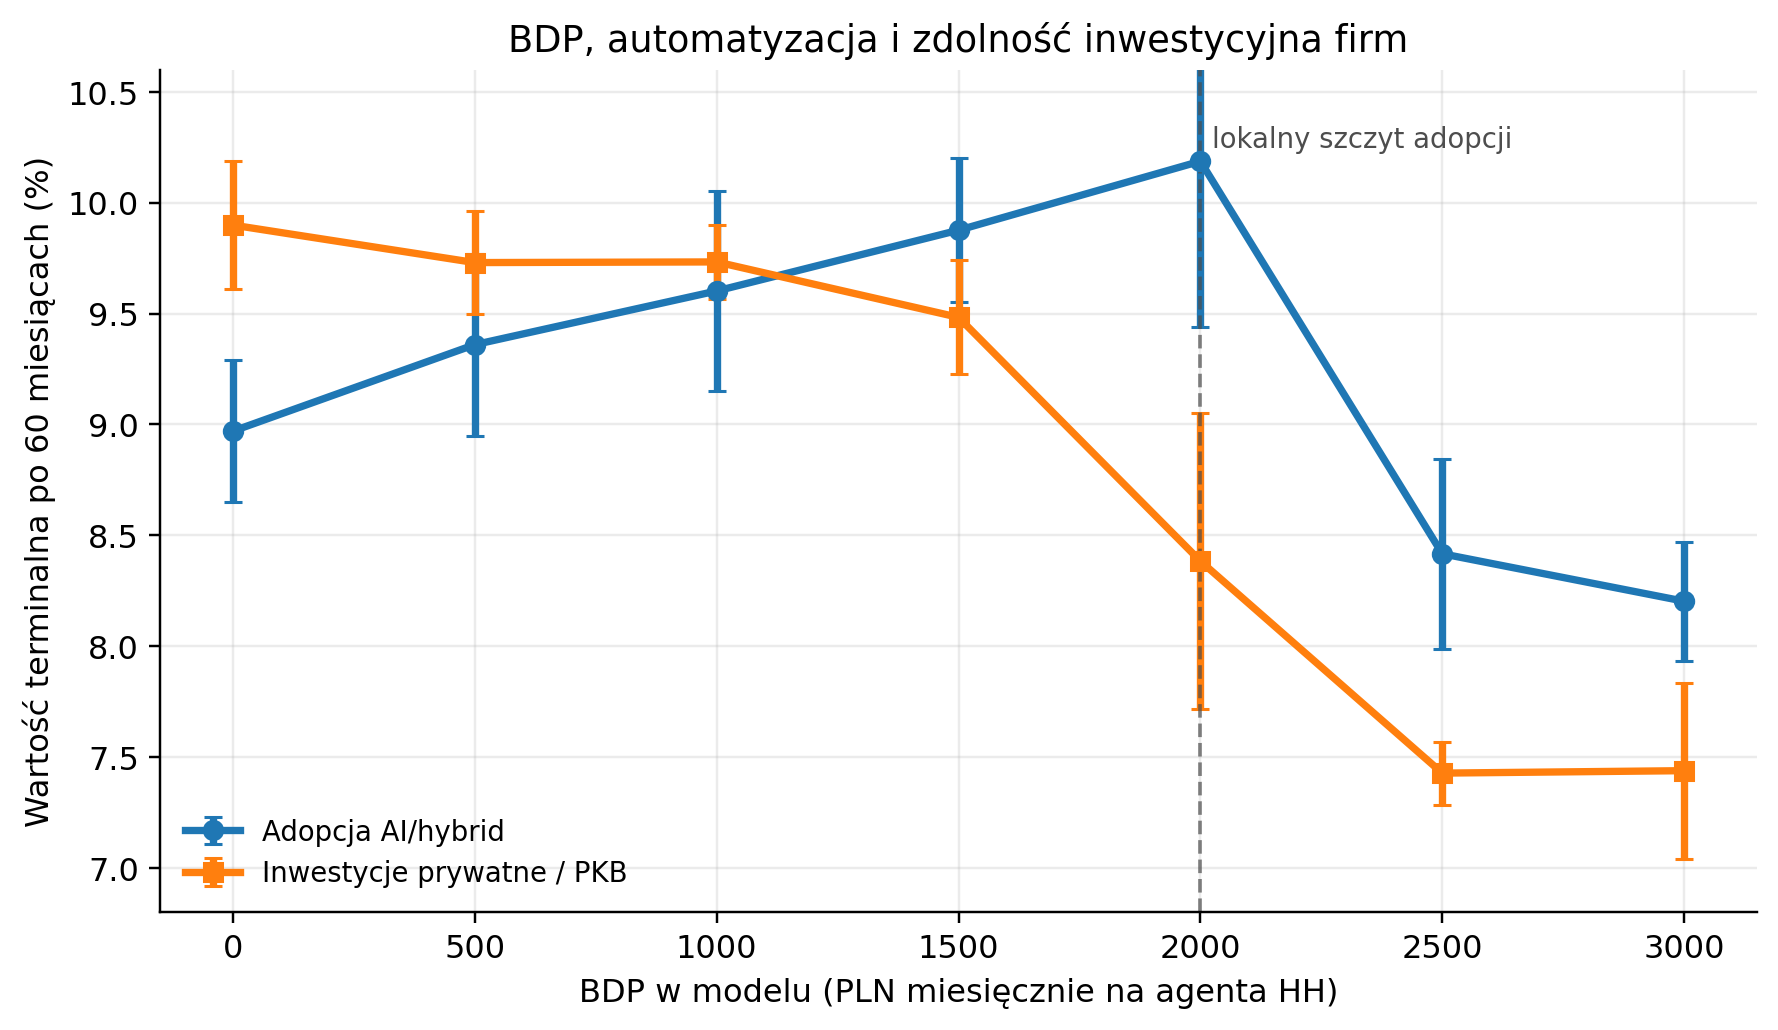
\includegraphics[width=\textwidth]{figures/fig01_bdp_adoption_investment.png}
  \caption{BDP, adopcja AI/hybrid i inwestycje prywatne. Punkty pokazują średnie terminalne dla 10 ziaren losowania, a pionowe odcinki pokazują odchylenie standardowe między ziarnami.}
  \label{fig:bdp-adoption-investment}
\end{figure}

\subsection{Odporność parametru lambda}

Analiza odporności pokazuje, że wynik nie jest czysto mechanicznym skutkiem samego transferu. Przy \(\lambda = 0\), czyli przy braku przełożenia BDP na płacę rezerwową, adopcja AI/hybrid pozostaje blisko wariantu bez BDP i nie tworzy wyraźnej krzywej akceleracji. Przy \(\lambda = 0{,}25\) adopcja rośnie łagodnie wraz z BDP, ale nie pojawia się gwałtowny próg. Oznacza to, że sam kanał popytowo-fiskalny nie wystarcza do mocnej wersji hipotezy.

Najwięcej mówi wariant centralny \(\lambda = 0{,}5\). Pokazuje on zakres umiarkowanego przyspieszenia adopcji: adopcja rośnie z 8,97\% w wariancie bez BDP do 10,19\% przy BDP 2000~PLN, a następnie spada do 8,42\% przy BDP 2500~PLN i 8,20\% przy BDP 3000~PLN. Warianty \(\lambda = 0{,}75\) i \(\lambda = 1\) przesuwają próg w lewo: lokalny szczyt pojawia się już przy BDP 1000~PLN, a wyższe poziomy transferu obniżają inwestycje prywatne i adopcję.

Wniosek z analizy odporności jest jednoznaczny: BDP może być katalizatorem automatyzacji tylko w przedziale pośrednim. Próg absorpcji wymaga jednoczesnej obecności presji płacowo-rezerwowej i kanału fiskalno-finansowego. Przy \(\lambda = 0\) rośnie deficyt i dług, ale adopcja AI/hybrid pozostaje blisko wariantu bez BDP; sam kanał fiskalny nie tworzy więc odwróconego U. Jeśli transfer wpływa na płacę rezerwową zbyt mocno, kanał kosztu pracy, inwestycji i finansowania zaczyna dławić zdolność firm do ucieczki technologicznej. Hipoteza ma więc charakter warunkowy, a nie monotoniczny.

\begin{figure}[H]
  \centering
  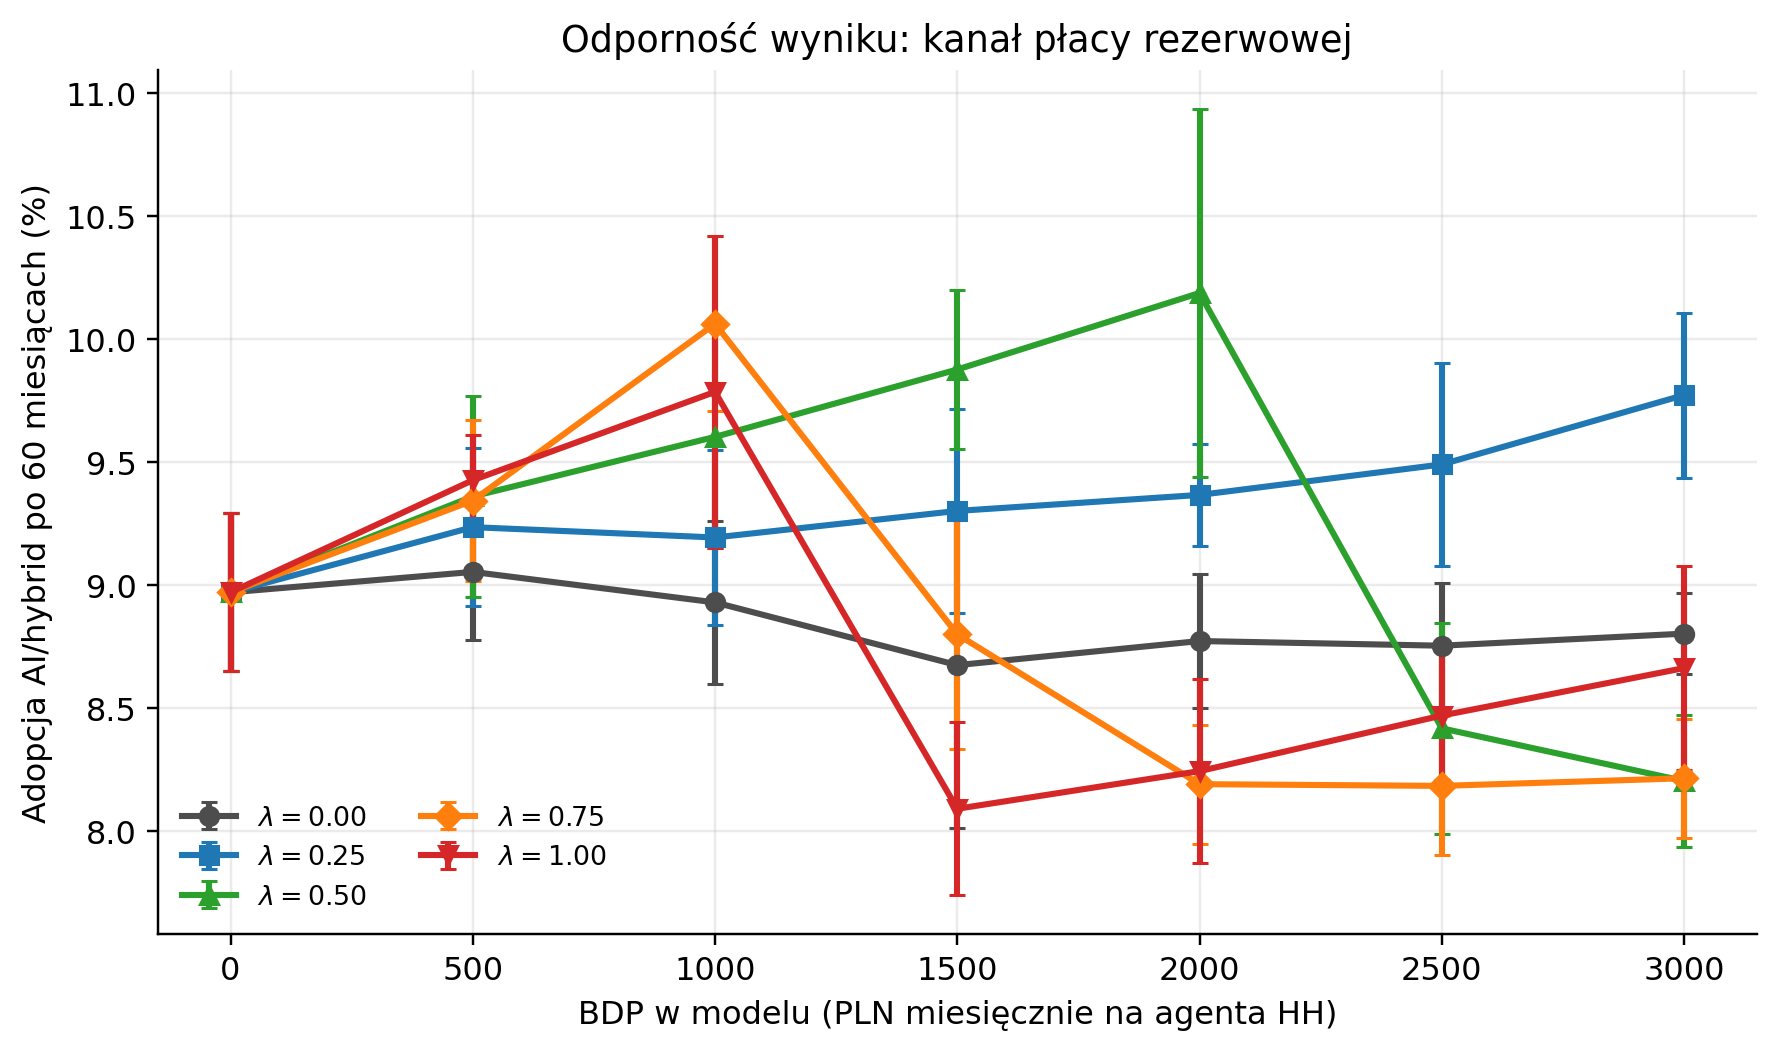
\includegraphics[width=\textwidth]{figures/fig05_lambda_robustness.png}
  \caption{Analiza odporności kanału płacy rezerwowej. Linie pokazują średnią terminalną adopcję AI/hybrid dla 10 ziaren losowania i pięciu wartości \(\lambda\).}
  \label{fig:lambda-robustness}
\end{figure}

\subsection{Ścieżka przejścia sektora firm}

Rysunek~\ref{fig:firm-transition-panel} pokazuje, co kryje się za wynikiem terminalnym. W wariancie BDP 2000~PLN adopcja AI/hybrid rośnie silniej niż w ścieżce bez BDP, ale dzieje się to przy wyraźnie słabszej ścieżce inwestycji prywatnych/PKB. Wysoki wariant BDP 3000~PLN pokazuje, że większa liczba firm nie oznacza automatycznie większej automatyzacji. Liczba aktywnych firm rośnie, ale inwestycje prywatne/PKB pozostają nisko, a adopcja AI/hybrid jest słabsza niż przy BDP 2000~PLN.

Nie jest to wyłącznie efekt wyższego mianownika PKB. W danych terminalnych spada także nominalny strumień prywatnych inwestycji brutto: z około 44,3 mld PLN miesięcznie w wariancie bez BDP do około 37,5 mld PLN przy BDP 2000~PLN i 33,9 mld PLN przy BDP 3000~PLN. W modelu inwestycja firmy jest ograniczana gotówką oraz możliwością pozyskania finansowania zewnętrznego. Wysoki BDP zwiększa deficyt i dług publiczny, podnosi rentowności obligacji publicznych oraz koszt długu korporacyjnego, a równocześnie przez kanał płacy rezerwowej i kursu walutowego pogarsza część kosztów firm. Presja automatyzacyjna rośnie, ale firmy mają mniej przestrzeni bilansowej, aby tę reakcję sfinansować. Ograniczeniem nie jest więc sama liczba podmiotów gospodarczych, lecz zdolność firm do finansowania inwestycji technologicznych.

\begin{figure}[H]
  \centering
  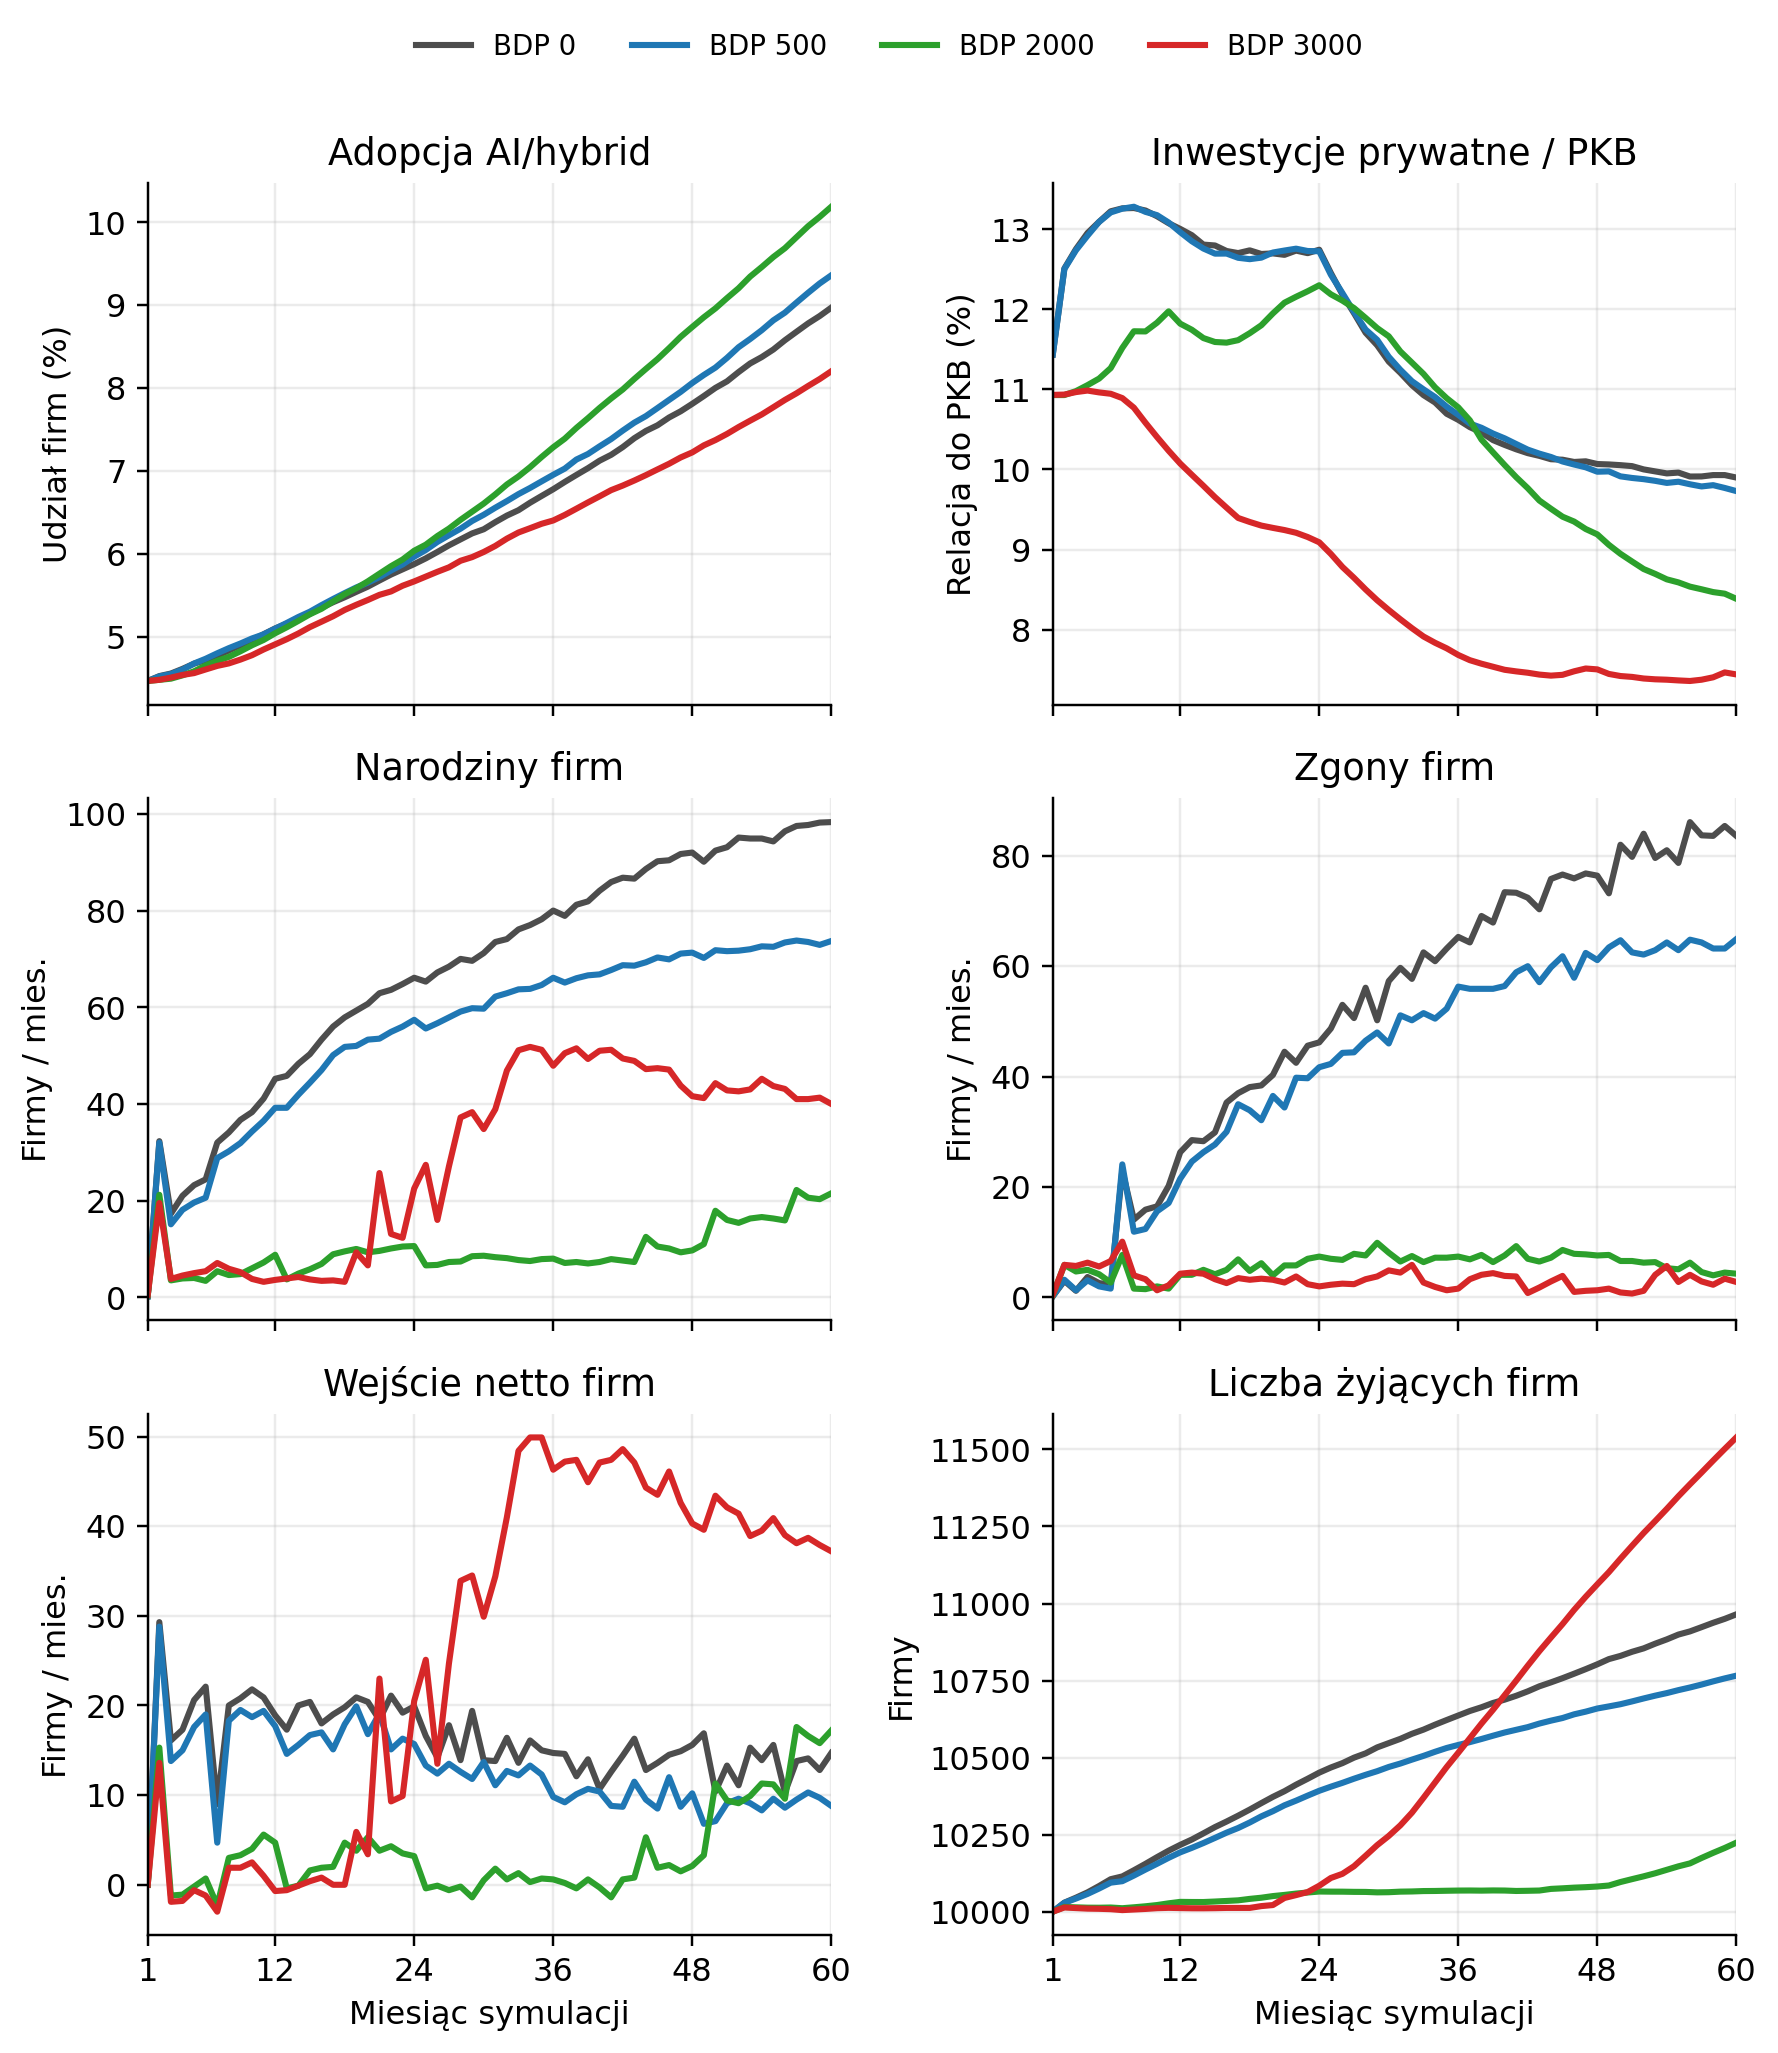
\includegraphics[width=\textwidth]{figures/fig06_firm_transition_panel.png}
  \caption{Ścieżki miesięczne sektora firm dla wybranych poziomów BDP. Linie pokazują średnie z 10 ziaren losowania: wariant bez BDP, dolną kotwicę BDP 500~PLN, wariant lokalnego szczytu adopcji BDP 2000~PLN oraz wysoki impuls BDP 3000~PLN.}
  \label{fig:firm-transition-panel}
\end{figure}

\begin{table}[H]
\centering
\scriptsize
\caption{Demografia firm i struktura wielkości w wariancie centralnym \(\lambda = 0{,}5\), miesiąc 60}
\label{tab:firm-demography-size}
\begin{tabular}{@{}r r r r r r r r@{}}
\toprule
\textbf{BDP} & \textbf{Aktywne} & \textbf{Nowe/mies.} & \textbf{Zamkn./mies.} & \textbf{Mikro \%} & \textbf{Małe \%} & \textbf{Średnie \%} & \textbf{Duże \%} \\
\midrule
0 & 10 965 & 98,3 & 83,6 & 90,87 & 8,23 & 0,71 & 0,19 \\
500 & 10 766 & 73,7 & 64,9 & 90,46 & 8,61 & 0,72 & 0,22 \\
1000 & 10 595 & 53,9 & 46,0 & 89,92 & 9,13 & 0,73 & 0,22 \\
1500 & 10 339 & 26,8 & 23,7 & 88,62 & 10,37 & 0,78 & 0,22 \\
2000 & 10 224 & 21,5 & 4,3 & 88,03 & 10,88 & 0,83 & 0,25 \\
2500 & 11 280 & 40,1 & 2,5 & 94,41 & 4,70 & 0,69 & 0,19 \\
3000 & 11 539 & 40,0 & 2,8 & 96,56 & 2,66 & 0,61 & 0,18 \\
\bottomrule
\end{tabular}
\end{table}


Dane o demografii firm uzupełniają ten wynik. Nie wskazują one na gwałtowną konsolidację rynku przez większe podmioty. W wariancie centralnym \(\lambda = 0{,}5\) pojawia się raczej nieliniowa zmiana struktury firm. Do poziomu BDP 2000~PLN spada zarówno liczba nowych firm, jak i liczba firm kończących działalność: z 98,3 nowych firm i 83,6 firm kończących działalność miesięcznie w wariancie bez BDP do 21,5 nowych firm i 4,3 firm kończących działalność miesięcznie. Jednocześnie udział mikrofirm spada z 90,87\% do 88,03\%, a udział firm małych rośnie z 8,23\% do 10,88\%. Można to interpretować jako zamrożenie selekcji rynkowej połączone z przejściem części firm poza mikrosegment.

Powyżej BDP 2500~PLN wzorzec się odwraca. Liczba firm rośnie do około 11,5 tys., ale wzrost ten odbywa się niemal wyłącznie w segmencie mikrofirm: ich udział wynosi 94,41\% przy BDP 2500~PLN i 96,56\% przy BDP 3000~PLN. Udział firm małych spada natomiast do 2,66\%. To nie jest obraz przejęcia rynku przez większych graczy. Bardziej prawdopodobna interpretacja to bariera skalowania i technologicznego dojrzewania sektora: nowe podmioty mogą powstawać jako mikrofirmy, ale przy wysokim koszcie kapitału i niższej inwestycji prywatnej trudniej im przejść do większych klas wielkości oraz sfinansować automatyzację.

\subsection{Płaca rezerwowa}

Kanał płacy rezerwowej jest aktywny mechanicznie: przy \(\lambda = 0{,}5\) scenariusz BDP 2000~PLN podnosi płacę rezerwową o 1000 PLN. Nie przekłada się to jednak natychmiast na silny wzrost płacy rynkowej. Modelowa płaca rynkowa pozostaje blisko wariantu bez BDP do poziomu BDP 1500~PLN, a wyraźniej rośnie dopiero przy BDP 2500~PLN i BDP 3000~PLN. Sam kanał płacy rezerwowej nie tłumaczy więc wzrostu adopcji AI/hybrid do BDP 2000~PLN.

\subsection{Popyt}

Transfer zwiększa dochód gospodarstw domowych, ale mediana konsumpcji i PKB reagują słabiej. Przy BDP 2000~PLN średni dochód gospodarstw rośnie względem wariantu bez BDP o około 2,1 tys. PLN, natomiast mediana konsumpcji tylko o około 190 PLN. Część impulsu trafia zatem do oszczędności, importu i bilansów, a nie wyłącznie do krajowego popytu finalnego.

\subsection{Panel kontrolny gospodarstw domowych}

Rysunek~\ref{fig:hh-control-panel} pełni funkcję kontroli alternatywnego wyjaśnienia. Gdyby nieliniowość adopcji AI/hybrid wynikała głównie z załamania sytuacji gospodarstw domowych, należałoby oczekiwać wyraźnej zmiany ubóstwa, nierówności albo niewypłacalności gospodarstw. W obecnym eksperymencie takiego sygnału nie widać. Średni dochód gospodarstw i mediana oszczędności rosną wraz z BDP, mediana konsumpcji rośnie umiarkowanie, a wskaźniki dystrybucyjne pozostają stabilne. Gini dochodowy pozostaje w przedziale około 0,28--0,29, stopa ubóstwa relatywnego 50\% mediany pozostaje blisko 13,5--14,3\%, a raportowana metryka bankructw gospodarstw domowych pozostaje zerowa w wariancie centralnym. Ten ostatni wskaźnik traktuję pomocniczo: model nie odtwarza administracyjnej procedury upadłości konsumenckiej, lecz służy do analizy kanałów makro-finansowych.

Ten panel zawęża interpretację wyniku. BDP poprawia płynność gospodarstw domowych, ale nie generuje w horyzoncie 60 miesięcy silnego szoku dystrybucyjnego, który sam tłumaczyłby próg automatyzacji. Nieliniowość adopcji należy więc wiązać przede wszystkim z interakcją kanału firmowego, płacowo-rezerwowego i fiskalno-finansowego: kosztem pracy, kosztem kapitału, inwestycjami prywatnymi oraz zdolnością firm do sfinansowania reakcji technologicznej.

\begin{figure}[H]
  \centering
  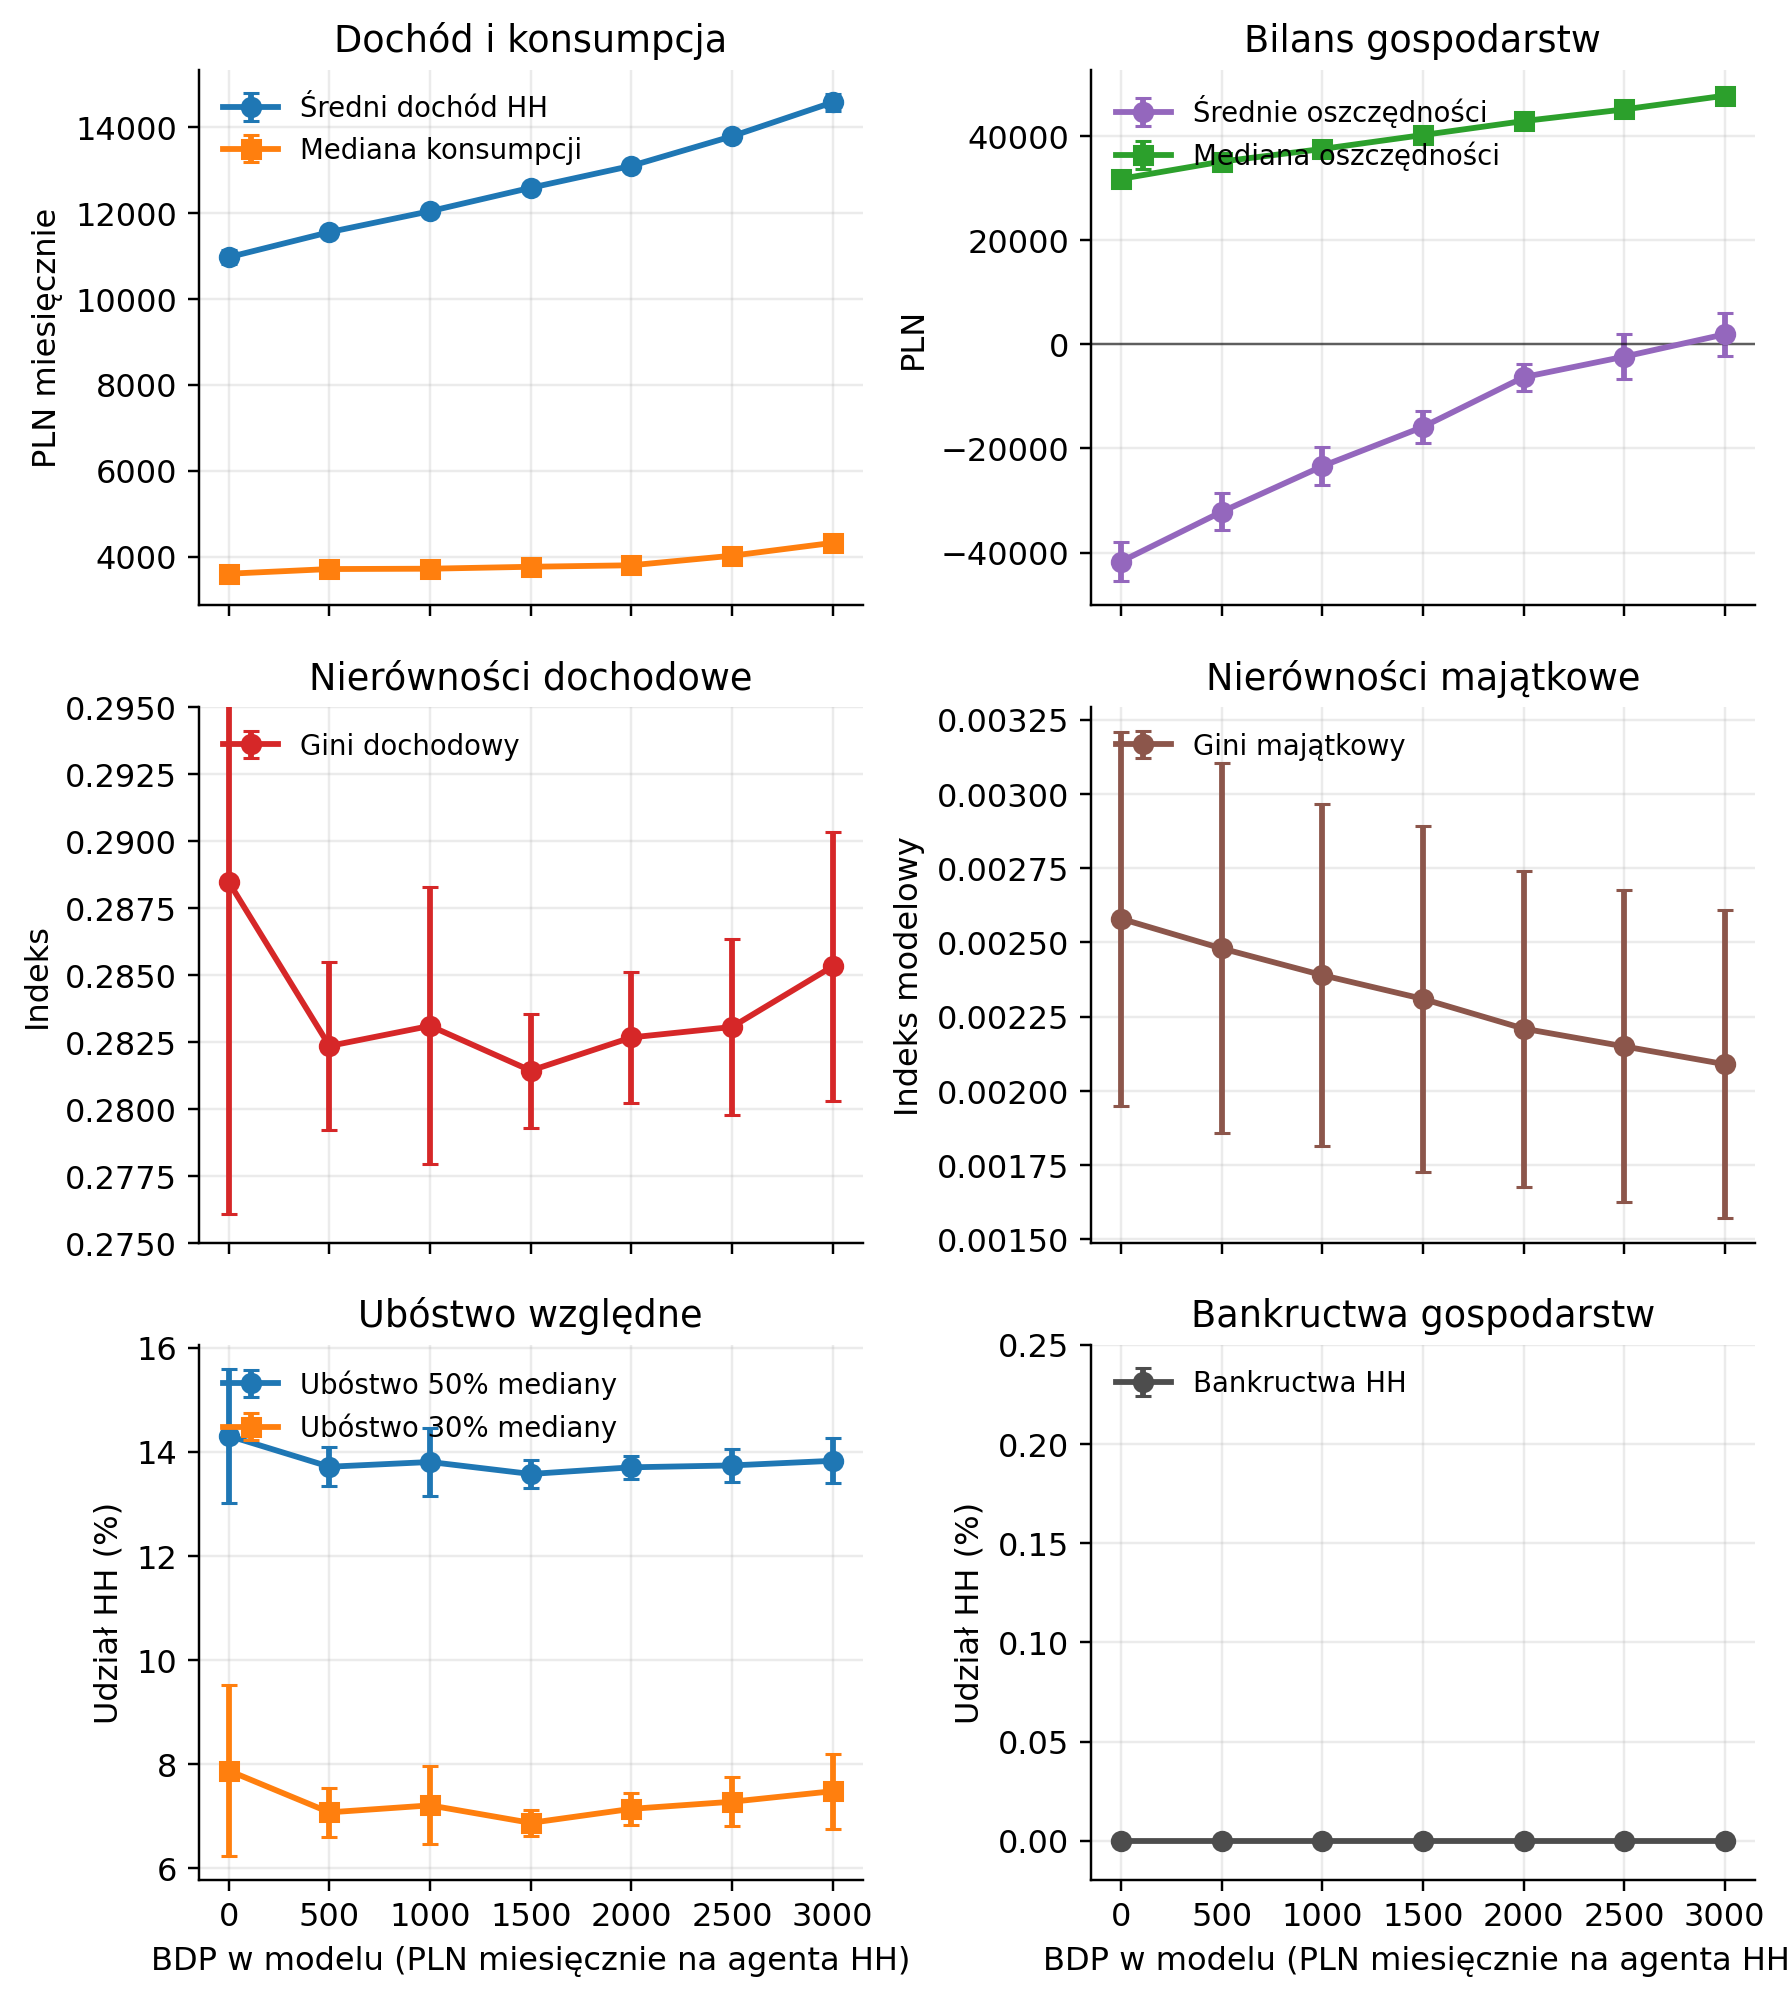
\includegraphics[width=\textwidth]{figures/fig07_hh_control_panel.png}
  \caption{Panel kontrolny gospodarstw domowych. Punkty pokazują średnie terminalne dla 10 ziaren losowania, a pionowe odcinki pokazują odchylenie standardowe między ziarnami.}
  \label{fig:hh-control-panel}
\end{figure}

\subsection{Inflacja i koszt kapitału}

Inflacja i stopa referencyjna NBP rosną umiarkowanie. Silniejszy sygnał pojawia się w koszcie finansowania rynkowego: rentowność obligacji i koszt długu korporacyjnego rosną wraz z poziomem BDP. To przesuwa interpretację z prostego kanału stopy NBP na kanał kosztu kapitału, obejmujący dług publiczny, obligacje korporacyjne i finansowanie inwestycji \parencite{blanchard2019}.

\begin{figure}[H]
  \centering
  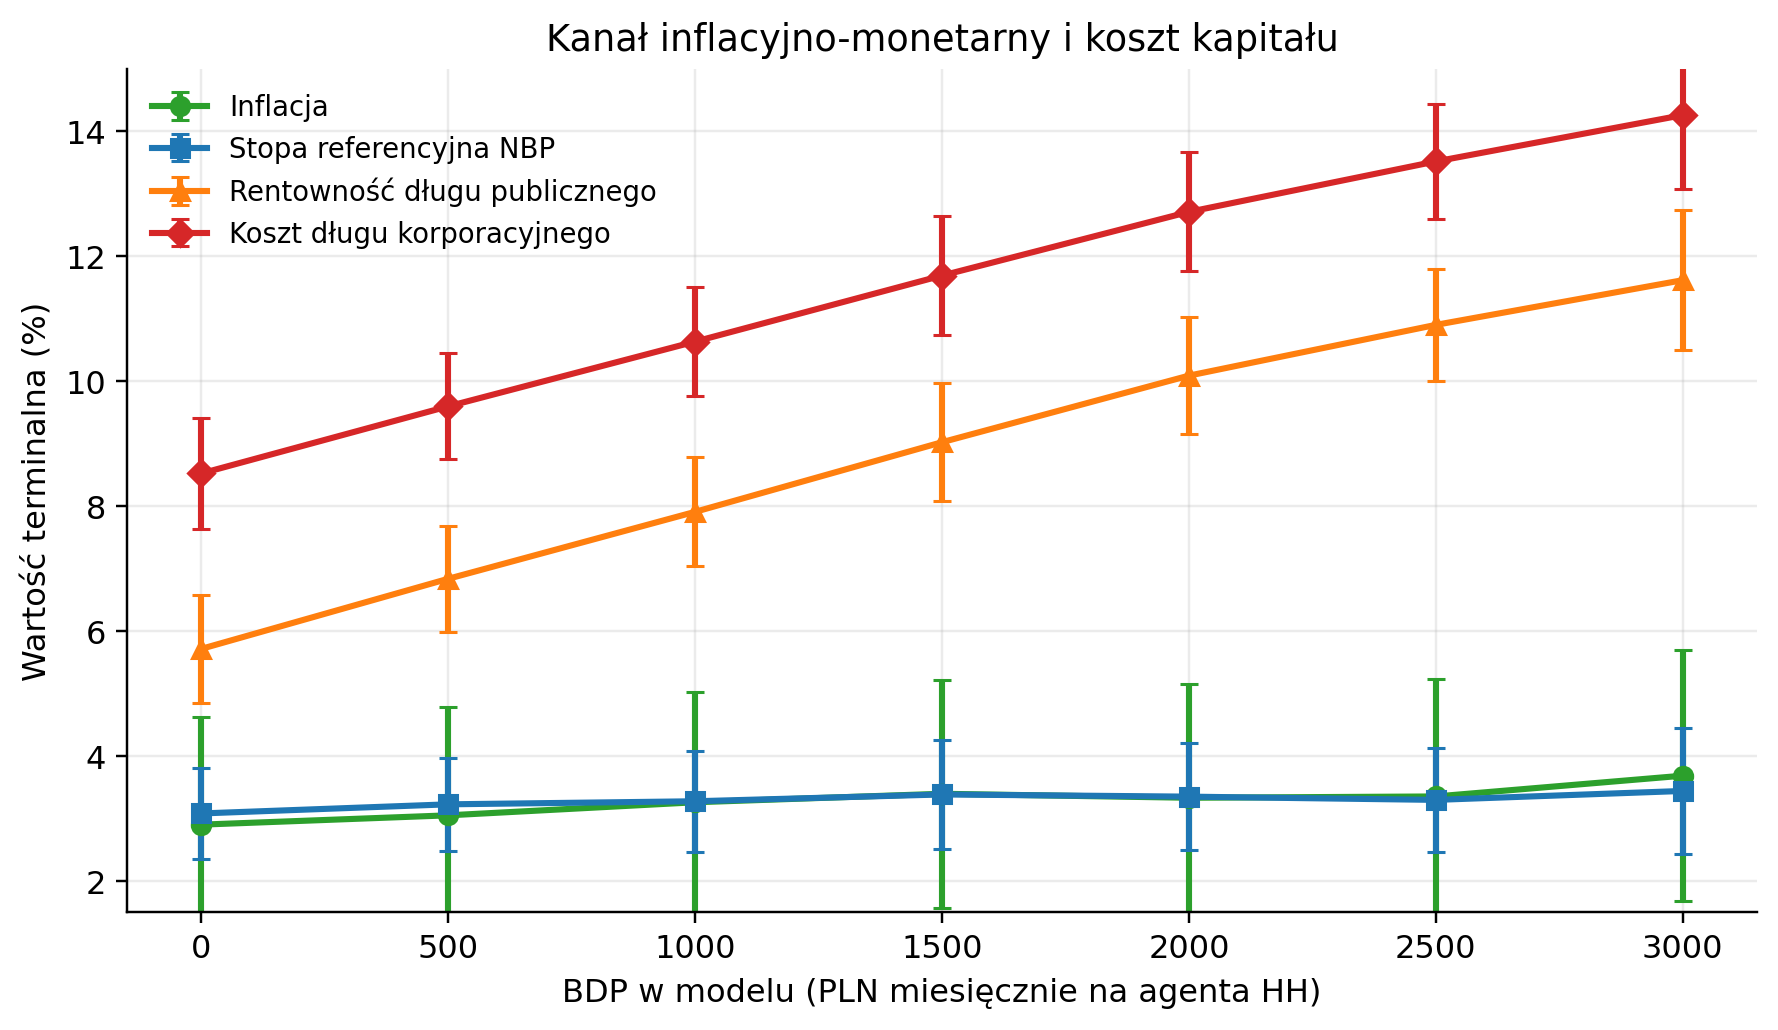
\includegraphics[width=\textwidth]{figures/fig03_bdp_cost_of_capital.png}
  \caption{Kanał inflacyjno-monetarny i koszt kapitału: inflacja, stopa NBP, rentowność długu publicznego i koszt długu korporacyjnego.}
  \label{fig:bdp-cost-capital}
\end{figure}

\subsection{Fiskus i dług}

Kanał fiskalno-dłużny jest najsilniejszy i monotoniczny \parencite{owsiak2017,mf2025debtStrategy,imf2026polandArticleIV}. Dług/PKB rośnie z 69,34\% w wariancie bez BDP do 97,12\% przy BDP 2000~PLN i 106,73\% przy BDP 3000~PLN. Deficyt/PKB rośnie z 7,69\% do odpowiednio 14,20\% i 16,55\%. W ujęciu różnicy względem wariantu bez BDP oznacza to wzrost długu o 27,77 pp PKB przy BDP 2000~PLN i 37,39 pp PKB przy BDP 3000~PLN; deficyt rośnie odpowiednio o 6,51 pp i 8,86 pp PKB. Przy wysokich poziomach transferu kanał fiskalno-dłużny zaczyna dominować nad pozytywnym kanałem popytowym, ale analiza \(\lambda = 0\) pokazuje, że sam wzrost deficytu i długu nie wystarcza do wyjaśnienia spadku adopcji AI/hybrid. Dla tej tezy decyduje interakcja z kanałem płacy rezerwowej i inwestycji firm.

\begin{figure}[H]
  \centering
  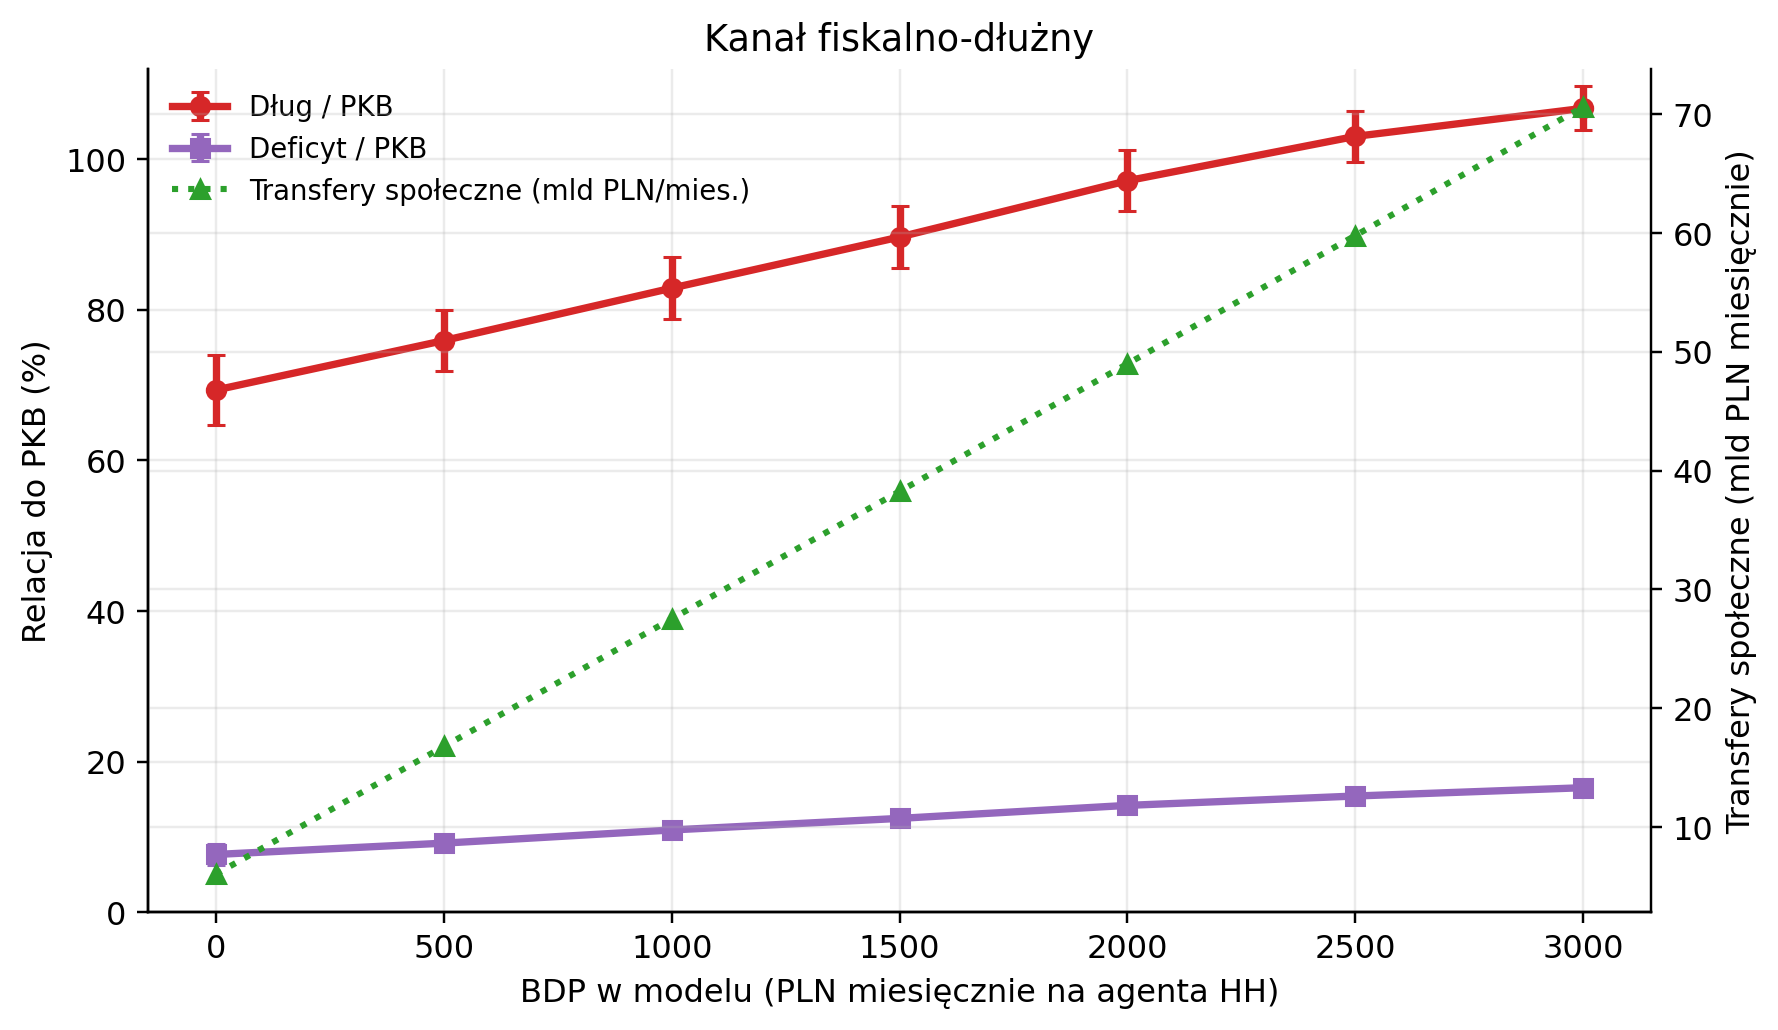
\includegraphics[width=\textwidth]{figures/fig02_bdp_fiscal_stress.png}
  \caption{Kanał fiskalno-dłużny: dług/PKB, deficyt/PKB oraz miesięczne transfery społeczne.}
  \label{fig:bdp-fiscal-stress}
\end{figure}

\subsection{Sektor zewnętrzny}

PLN słabnie, import rośnie, a rachunek bieżący pogarsza się. Przy BDP 3000~PLN kurs PLN/EUR jest o około 3,2\% wyższy niż w wariancie bez BDP, import o około 6,5\% wyższy, a rachunek bieżący pogarsza się o około 3,22 pp PKB względem ścieżki bez BDP. Część impulsu popytowego odpływa więc przez import i kanał kursowy.

\begin{figure}[H]
  \centering
  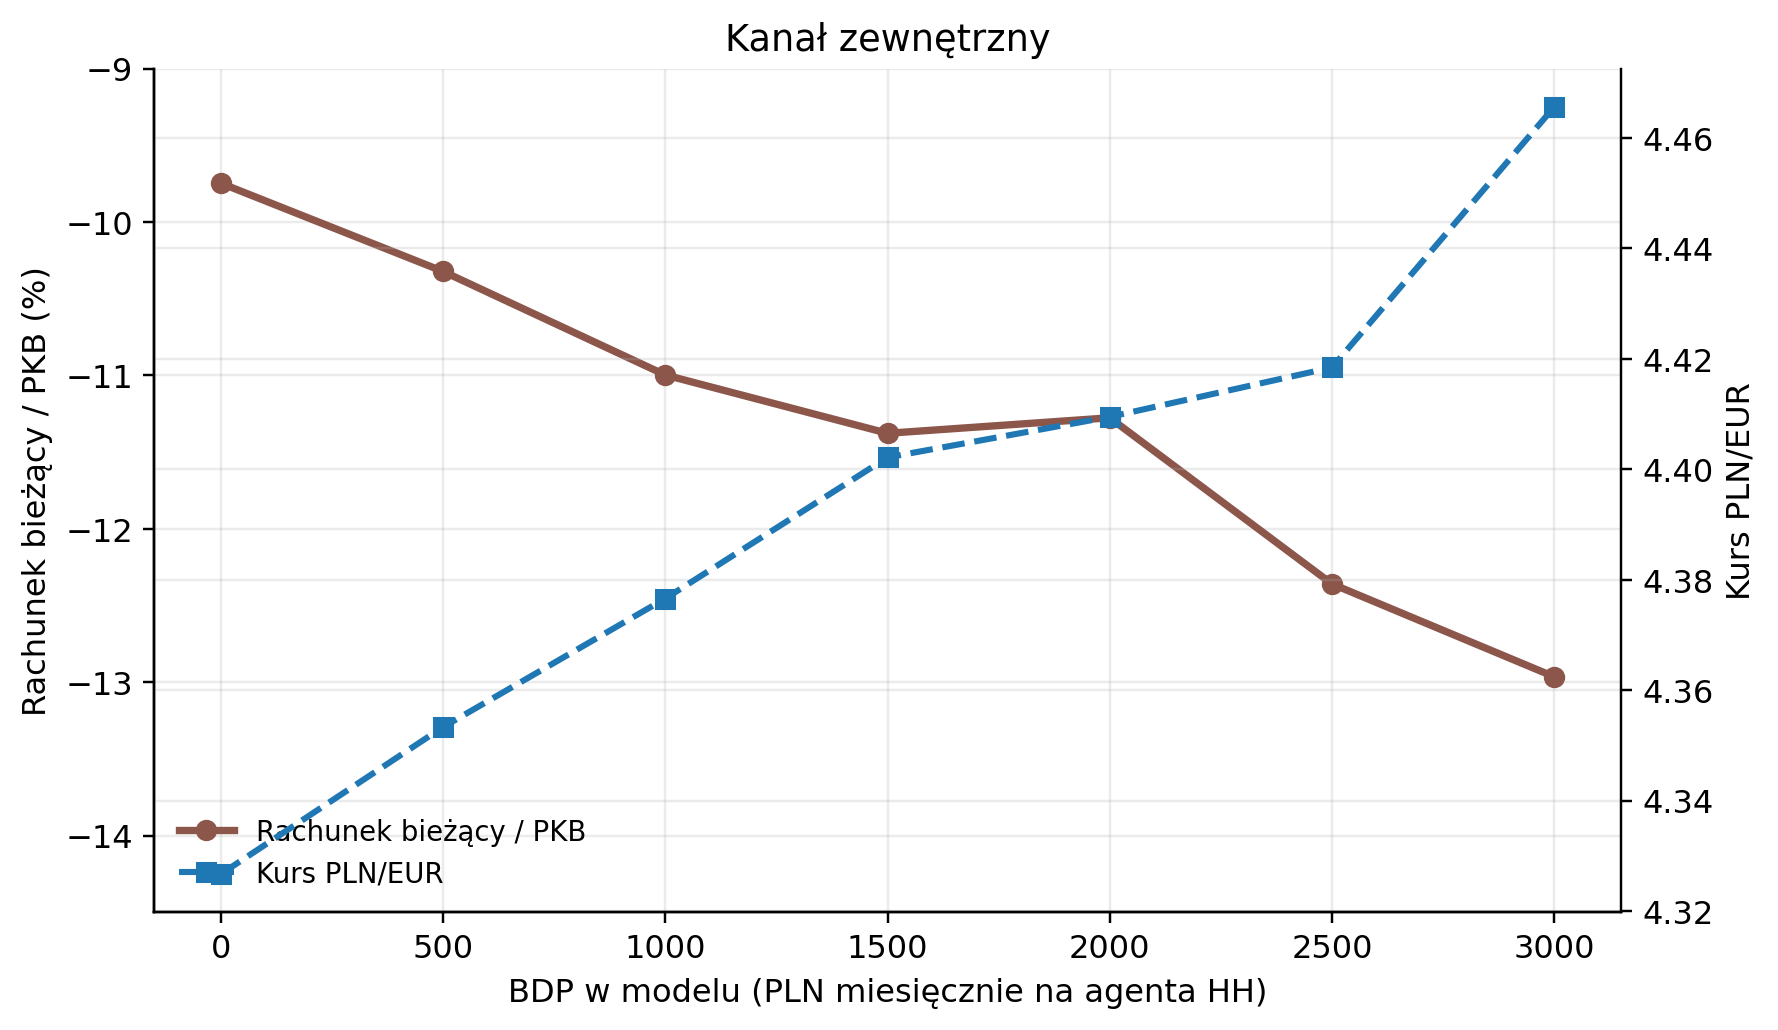
\includegraphics[width=\textwidth]{figures/fig04_bdp_external_channel.png}
  \caption{Kanał zewnętrzny: rachunek bieżący do PKB oraz kurs PLN/EUR.}
  \label{fig:bdp-external-channel}
\end{figure}

\subsection{Kredyt i banki}

W eksperymencie nie widać kryzysu bankowego. Nie występują upadłości banków, wskaźniki CAR/LCR/NSFR pozostają wysokie, a NPL nie rosną monotonicznie. Ograniczenie automatyzacji przy wysokim BDP nie wynika z załamania sektora bankowego, lecz raczej z pogorszenia opłacalności i zdolności finansowania inwestycji prywatnych.

\subsection{Automatyzacja i inwestycje}

Adopcja AI/hybrid rośnie do BDP 2000~PLN, ale równolegle prywatne inwestycje/PKB spadają z 9,90\% w wariancie bez BDP do 8,38\%. Przy BDP 2500~PLN i BDP 3000~PLN inwestycje prywatne/PKB spadają do około 7,4\%, a adopcja AI/hybrid obniża się poniżej wariantu bez BDP. To wskazuje na próg absorpcji w wariancie deficytowym: firmy mogą reagować automatyzacją tylko tak długo, jak mają zdolność finansowania tej reakcji i jednocześnie odczuwają presję po stronie płacy rezerwowej.

Dlatego eksperyment wspiera wersję warunkową hipotezy. Deficytowo finansowany BDP może przyspieszać automatyzację w przedziale, w którym presja kosztowa i popytowa nie ograniczają zdolności inwestycyjnej sektora prywatnego. Po przekroczeniu progu wynikającego z interakcji presji płacowo-rezerwowej oraz ograniczeń fiskalno-finansowych gospodarka nie przechodzi do szybszej automatyzacji, lecz do niższej dynamiki inwestycji prywatnych, pogorszenia bilansu zewnętrznego i silniejszego obciążenia długu publicznego.
